% LaTeX schematics: Current Source
% Description: DC Current Source connected to Elmer Massive Coil
% Author: Jonathan Velasco, CSC - IT Center for Science
% Original date: September 2021
% email: jonathan.velasco@csc.fi
%------------------------------------------------------

%------------------------------------------------------
%         Document Settings
%------------------------------------------------------
\documentclass
[border=3mm]{standalone}

%------------------------------------------------------
%         Packages
%------------------------------------------------------

\usepackage[siunitx,cuteinductors,americanvoltages,americancurrents]{circuitikz}  

%------------------------------------------------------
%         Main
%------------------------------------------------------
\begin{document}     
        \begin{circuitikz}[PH/.append style={font=\scriptsize,inner ysep=2pt,inner xsep=5pt},
                           PV/.append style={PH,inner ysep=2pt,inner xsep=2pt}]
                           
           \node[inner sep=0pt] (whitehead) at (2, 4) % (8.5,2) 
                    {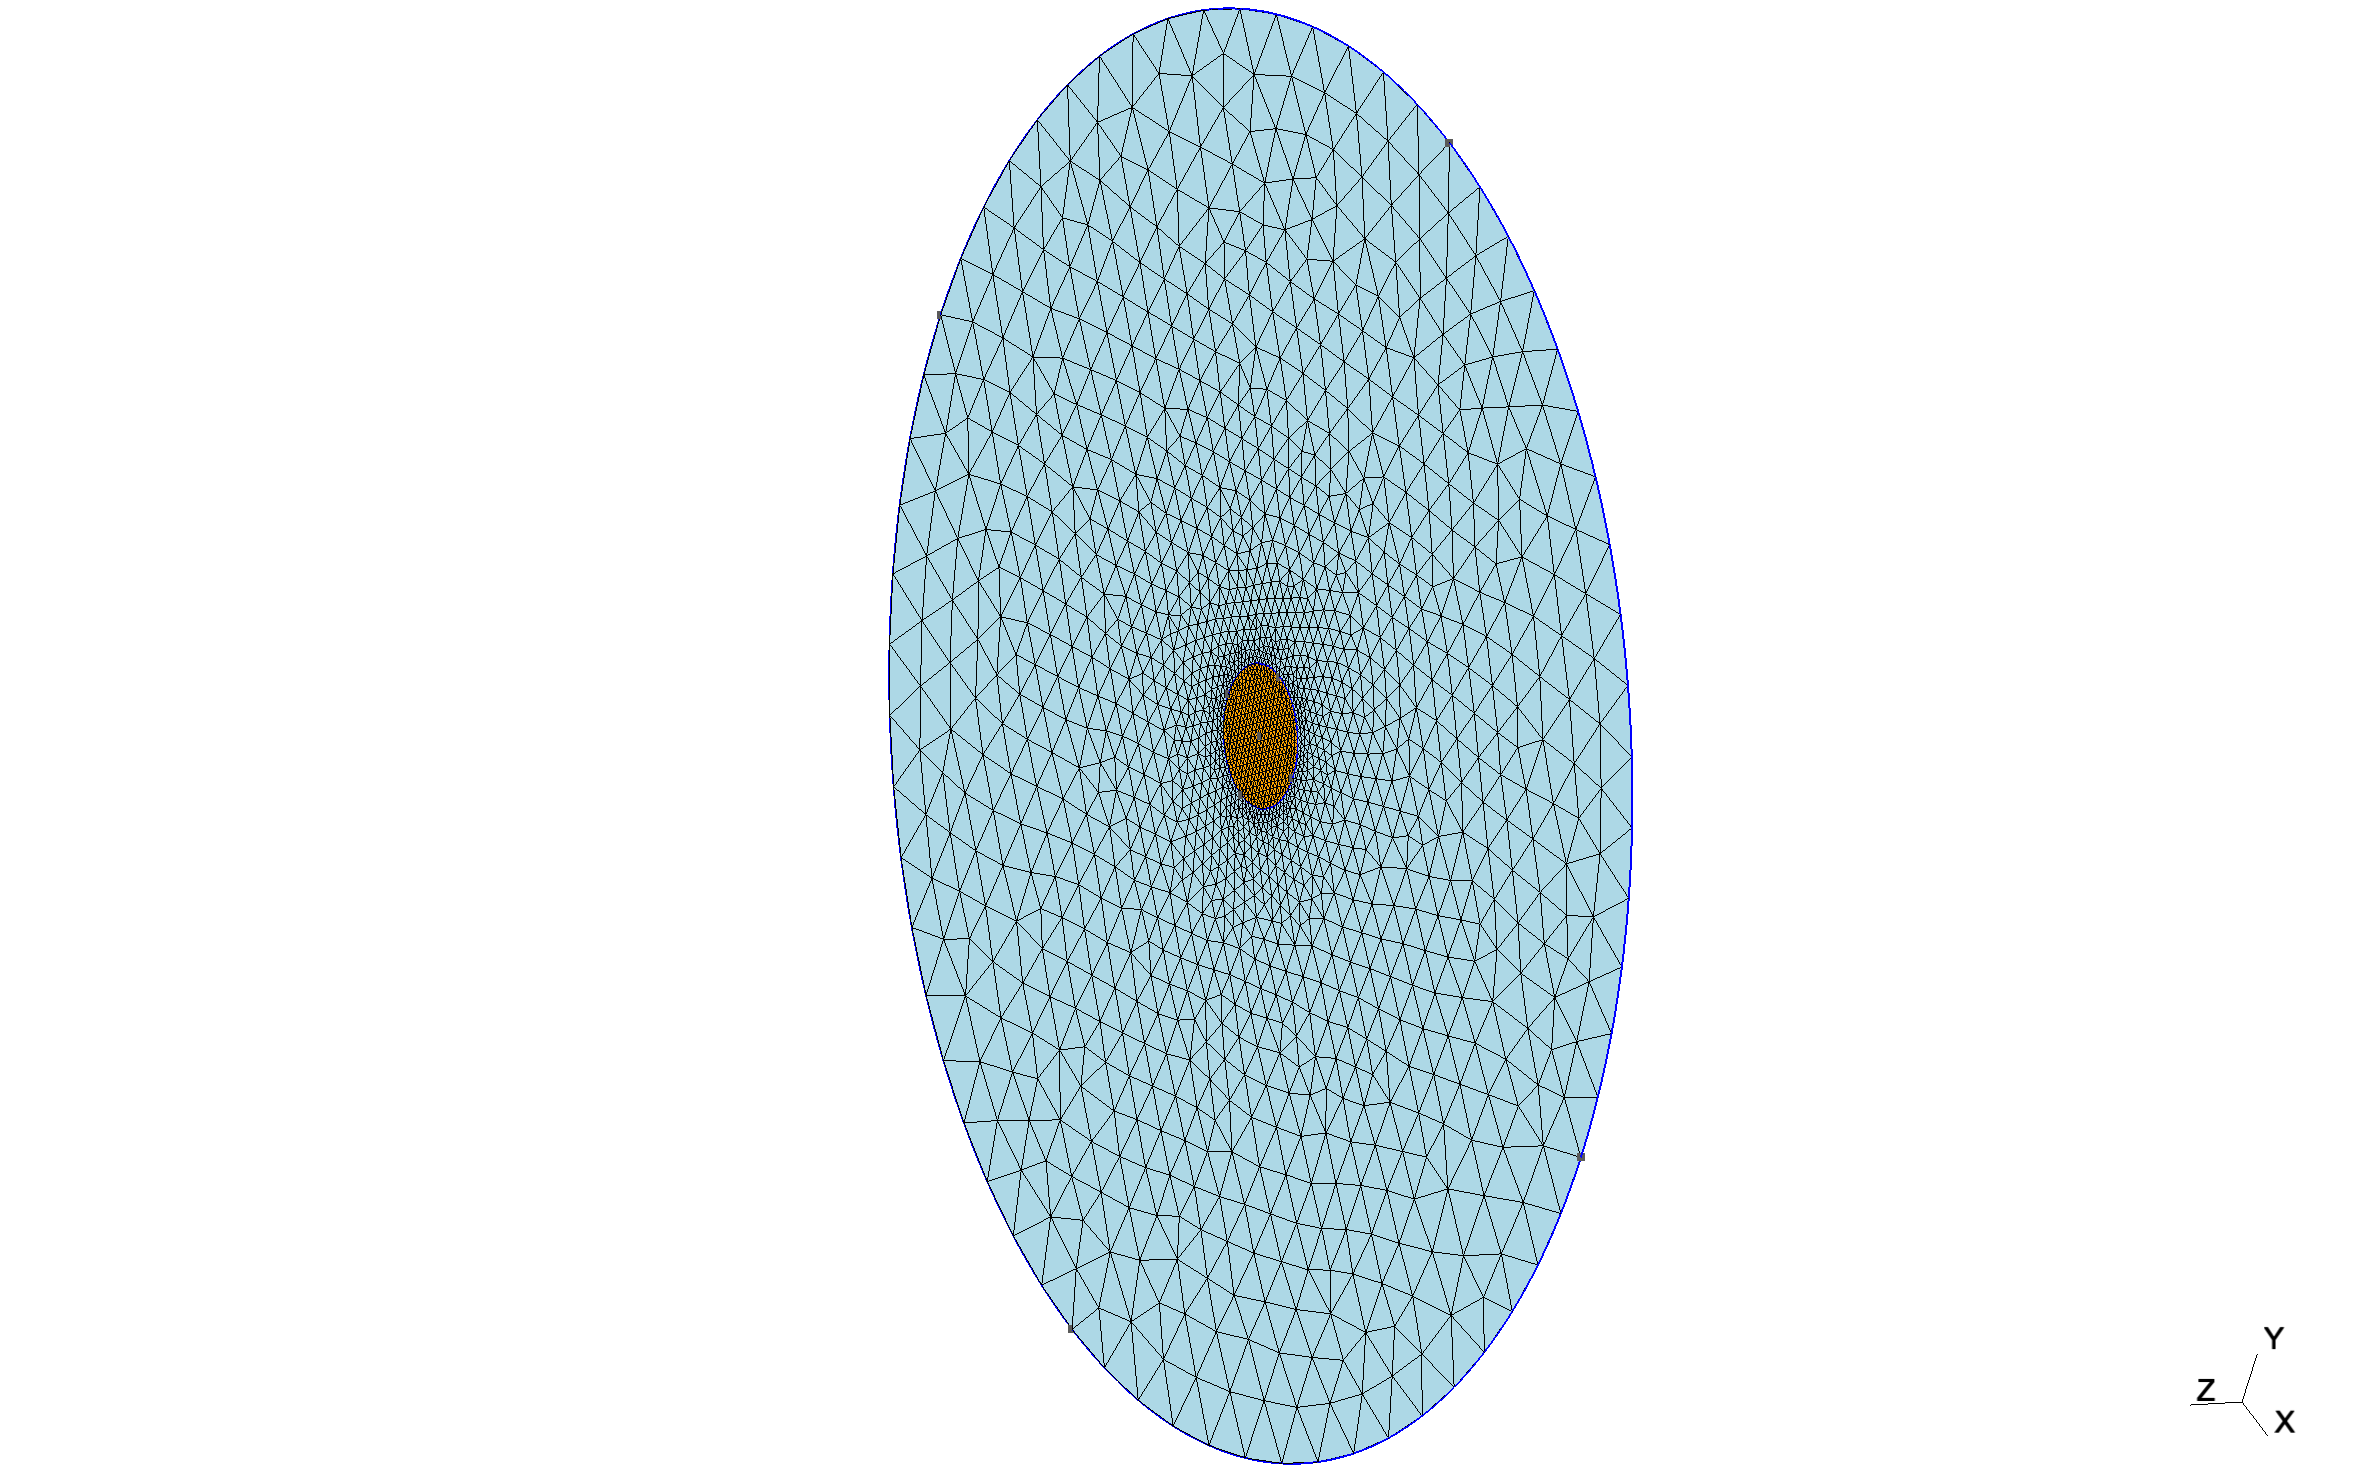
\includegraphics[width=.7\textwidth]{../tex-models/figures/wire2D_mesh.png}};
                
                \draw (0,0) % Begin Circuit
                
                % Ideal DC Voltage Source
                to[I ,name=Is,-,l^=$\mathbf{I_{s_1}^{ckt_1}}$, v^={$$},thick] (0,4) (0,0)
                
%                % Elmer FEM Component
%                (0,4) node [PV,above left] {2} 
%                to[generic, l^=$\mathbf{ElmerComponent}$,name=Ecomp,*-]  (4,4) 
                
                % Short Wires
                 (0,4) node [PV,above left] {2}  to[short,*-] (2.25,4) 
                 (3.62,4) to[short,-] (4, 4) 
                 (4,4) 
                to[short,-] (4,0) 
                to[short,-] (2,0) node [ground]{} node [PV,above left] {1} (2,0) 
                to[short,*-] (0,0) ;
                
                % Component Values
                \node[above, xshift=31pt, yshift=-14pt] at (Is.n) {1A};
                %\node[below, xshift=2pt, yshift=-14pt] at (Ecomp.n) {Massive Coil};
                 \node[below, scale = 2.5] at (2.5,3){$\Omega_{c}^{C}$};
               \draw [->, thick] (4,5) -- (2.25,4);
                \node[below, scale = 2.5] at (5,5.6){$\Omega_{c_1}^{ckt_1}$};


        \end{circuitikz}
\end{document}

%------------------------------------------------------
%         EOF
%------------------------------------------------------